\begin{table}
    \centering
    \begin{tabular}{|l|l|l|l|l|l|l|l|l|}
    \hline
        Index & Layers & Act. & Loss & Epochs & Alpha & Beta & Acc.\(\%\) & MCE \\ \hline
        1132 & 21-15-20-3 & ISRLU & SSE & 500 & 0.01 & 0.95 & 100.00 & 0.1819 \\ \hline
        1120 & 21-15-20-3 & ISRLU & SSE & 500 & 0.01 & 0.5 & 100.00 & 0.1827 \\ \hline
        1048 & 21-15-20-3 & ISRLU & MSE & 500 & 0.01 & 0.5 & 100.00 & 0.1835 \\ \hline
        1067 & 21-20-45-3 & ISRLU & MSE & 300 & 0.01 & 0.95 & 100.00 & 0.1835 \\ \hline
        1049 & 21-20-45-3 & ISRLU & MSE & 500 & 0.01 & 0.5 & 100.00 & 0.1836 \\ \hline
        30 & 21-12-3 & ISRLU & CEE & 500 & 0.01 & 0.95 & 100.00& 0.1838 \\ \hline
        31 & 21-15-3 & ISRLU & CEE & 500 & 0.01 & 0.95 & 100.00& 0.1838 \\ \hline
        33 & 21-12-3 & ISRLU & CEE & 300 & 0.01 & 0.95 & 100.00& 0.1838 \\ \hline
        240 & 21-12-3 & ISRLU & SSE & 500 & 0.01 & 0.95 & 100.00 & 0.1838 \\ \hline
    \end{tabular}
\end{table}


\begin{figure}
    \centering
    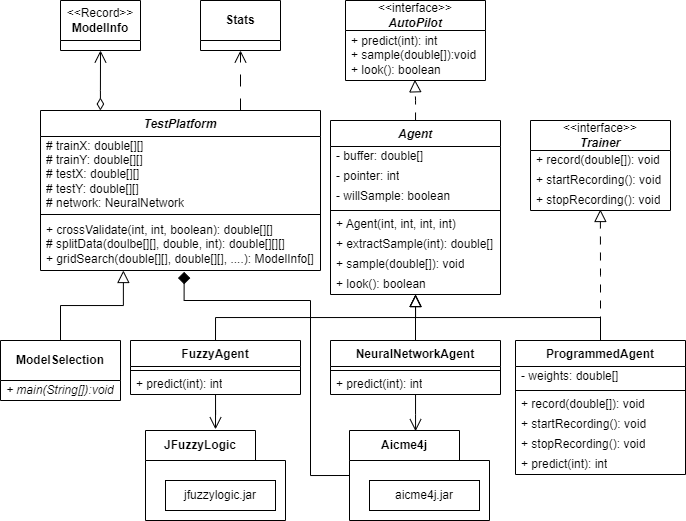
\includegraphics[width=\linewidth]{uml.png}
    \caption{UML Diagram}
    \label{fig:uml}
\end{figure}

\begin{figure}
    \centering
    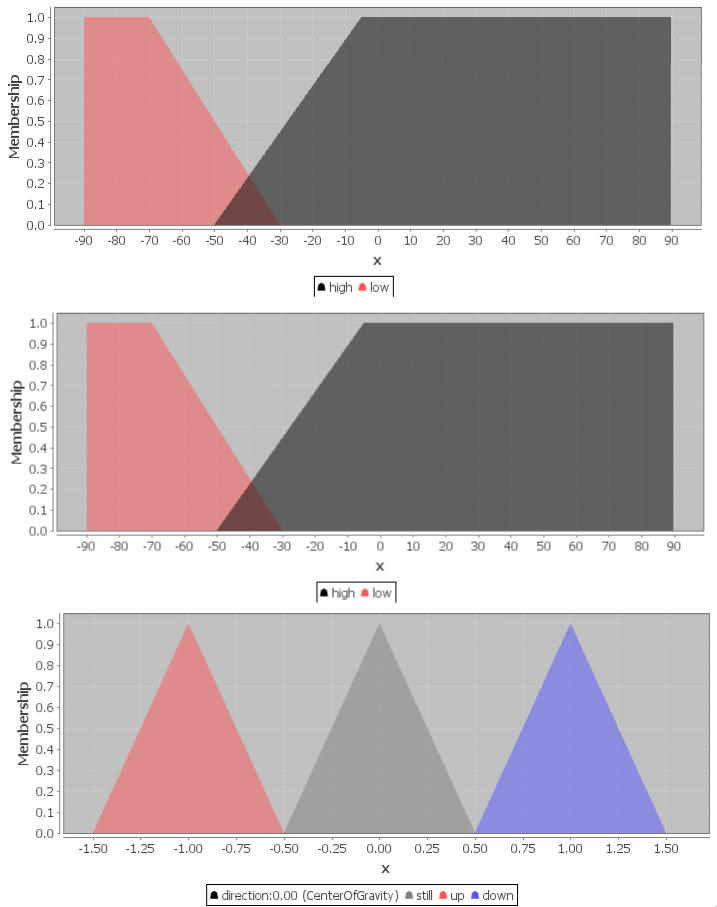
\includegraphics[width=\linewidth]{fzzy.png}
    \caption{Membership Functions}
    \label{fig:fuzzy}
\end{figure}